\chapter{Background}\label{Background}

This chapter offers an overview of the technology and concepts needed to understand the context and relevance of the work within the broader world. The review is conducted predominately through a networking, security and privacy perspective to best highlight the aspects pertinent to the distributed deployment of ECH. This chapter also represents the bulk of the effort put into investigating and studying the functioning of ECH while identifying and experimenting with different deployment models.

The contents of this chapter include a high level description of the Transport Layer Security protocol and the Domain Name System with a more detailed look at the components that enable ECH functionality. This is followed by an inspection of ECH itself, its security properties and the mechanisms which allow for distributed deployment. Finally, we survey how a variety of traffic analysis techniques that can be used to infer sensitive information from patterns in network activity, as well as the countermeasures which exist to mask these patterns.








\section{Transport Layer Security}

Transport Layer Security (TLS) is a cryptographic protocol proposed by the Internet Engineering Task Force (IETF) which enables secure network communication over public networks. Applications and services can establish an encrypted communication channel to transmit private information such that confidentiality, integrity and authenticity of the data can be ensured. TLS is commonly used to protect Internet traffic, having seen widespread adoption and several revisions since its original inception in 1999, superseding the Secure Sockets Layer (SSL) specification previously defined by Netscape Communications from 1994~\cite{chan2018monitoring, LE-HTTPS, rfc2246}.

TLS is designed to operate on top of a reliable transmission protocol between a client and server, such as the Transmission Control Protocol (TCP) when used over the Internet. In order to prevent eavesdropping, tampering and message forgery, TLS includes a number of security features based on a number of cryptographic mechanisms:

\begin{description}
	\item[Confidentiality:] All service and application data exchanged between the client and server is encrypted as to make it indecipherable to any intermediate party which might be intercepting their communication. For example, consider the importance of protecting customer passwords and banking information when accessing financial services.
	\item[Data integrity:] In a similar manner, cryptographic properties are used to guarantee transferred data cannot be modified during transmission. This is critical for safeguarding against input manipulation in consequential situations, such as while conducting a monetary transaction.
	\item[Authentication:] TLS provides the ability for both participants to verify the identity of the other, ensuring privileged communication is only performed with the intended recipient. Such a condition is fundamental for establishing trust and confidence in sensitive environments, as is required when interacting with online financial institutions.
\end{description}

TLS 1.3 is the latest defined standard for the protocol, having been published in August 2018 and contributing to the deprecation of TLS 1.0 and TLS 1.1 in March 2021~\cite{rfc8446, rfc8996}. It introduces many major changes to TLS 1.2, including the addition of a zero round trip time resumption (0-RTT) mode, further encryption and optimisation of the handshake and removal of outdated cryptographic algorithms and security mechanism with all key exchanges now providing forward secrecy. A change of particular relevance to ECH is the encryption of the server certificate received by the client to authenticate the server. Without this, the identity of the server is apparent to all observers so ECH would be far less valuable. Let us now examine <these>

\subsection{Digital Certificates}

TLS uses digital certificates to make assertions on the identity of entities within the network. These certificates contain <> which enables , provided a number of <steps>

% These certificates are exchanged during the TLS handshake,  of secure communication between the client and server to . Their <functioning> is based on a number
%
% They serve as a crucial component of the TLS handshake process, enabling both parties to authenticate each other's identity and establish a secure communication channel

<public key, trust>

\begin{figure}[ht]
\centerline{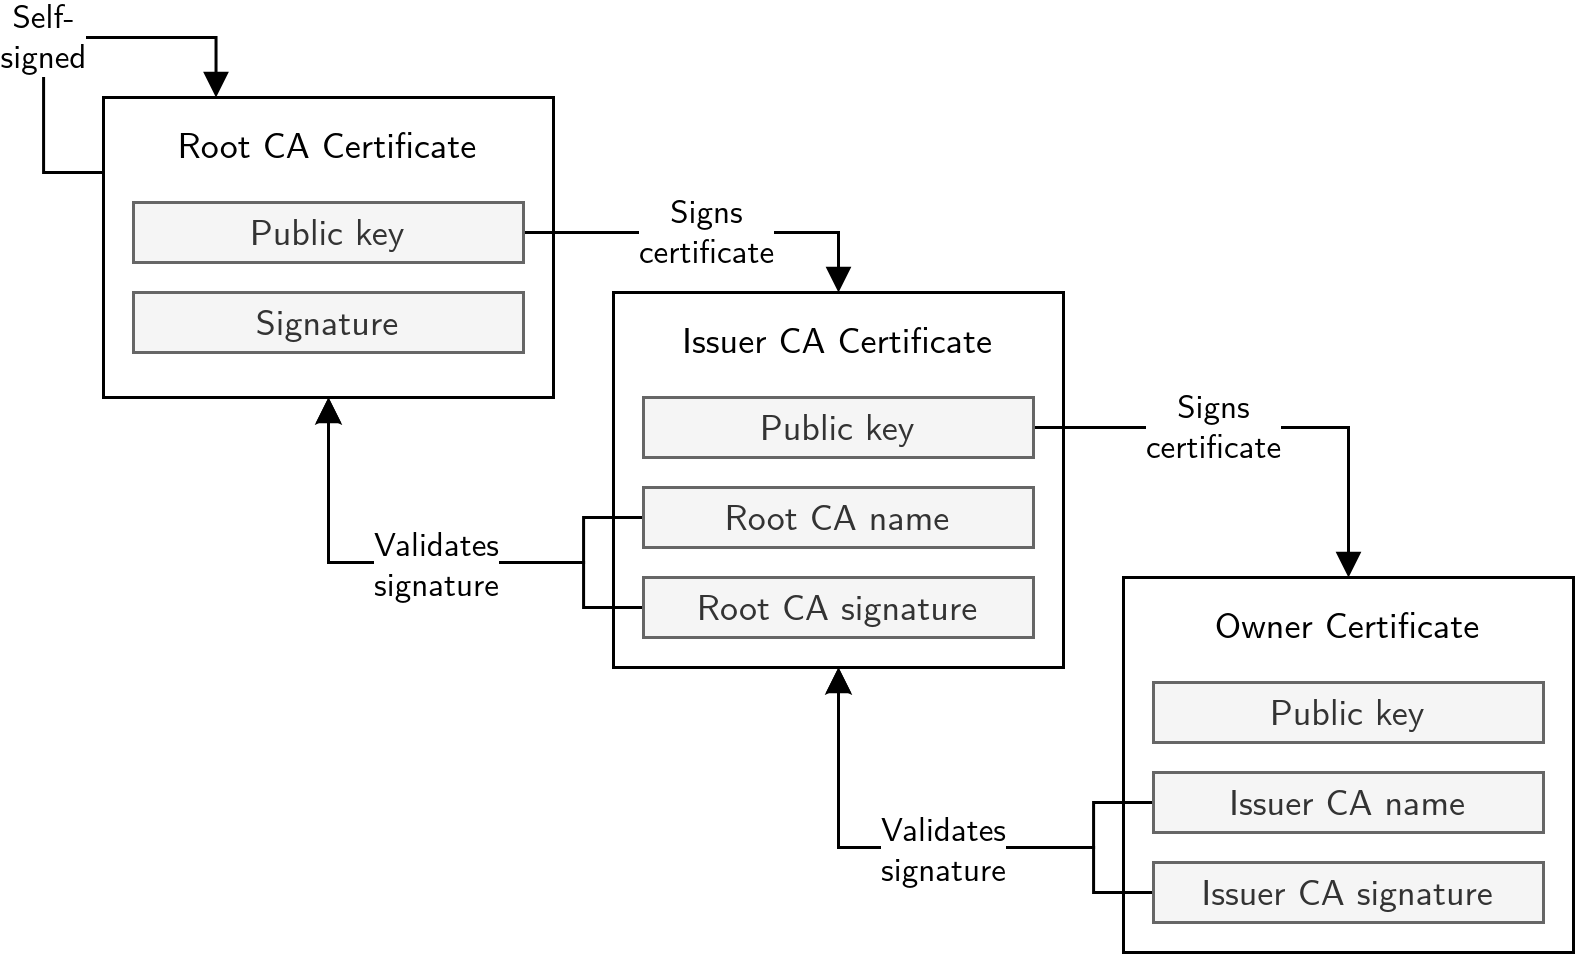
\includegraphics[width=160mm]{images/tls-chain.png}}
\caption[TLS certificate chain of trust]{<>}
\label{tls_chain_figure}
\end{figure}

\subsection{Handshake}

\begin{figure}[ht]
\centerline{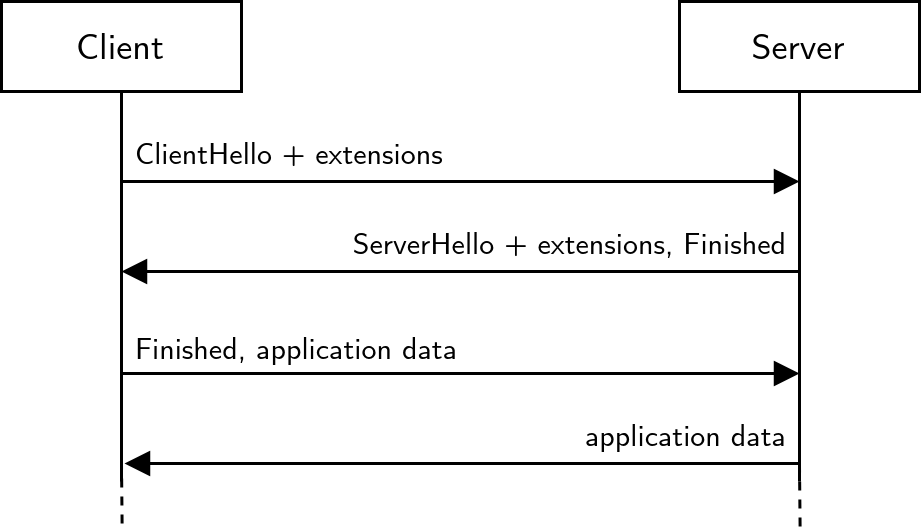
\includegraphics[width=120mm]{images/tls-handshake.png}}
\caption[Basic TLS 1.3 handshake]{<>}
\label{tls_handshake_figure}
\end{figure}

\begin{description}
	\item[ClientHello] <>
	\item[ServerHello] <>
\end{description}

<application data>

\subsection{Extensions}

<is>
<greasing>








\section{The Domain Name System}

<is>
<purpose>

\subsection{Name Resolution Process}

<>

\begin{figure}[ht]
\centerline{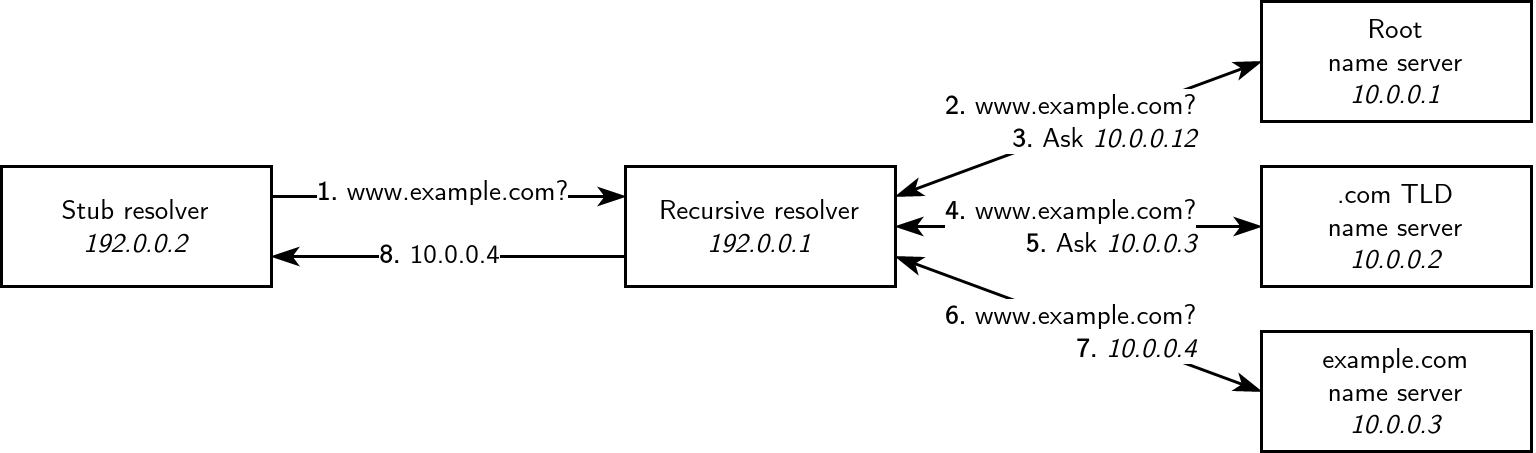
\includegraphics[width=160mm]{images/dns-resolve.png}}
\caption[Example DNS name resolution process]{<>}
\label{dns_resolve_figure}
\end{figure}

\subsection{DNS Over HTTPS}

\blindtext

\subsection{The HTTPS Resource Record}

\blindtext








\section{Encrypted Client Hello}

\blindtext

\subsection{Hybrid Public Key Encryption}

\blindtext

\subsection{Split Mode Deployment}

\blindtext

\begin{figure}[ht]
\centerline{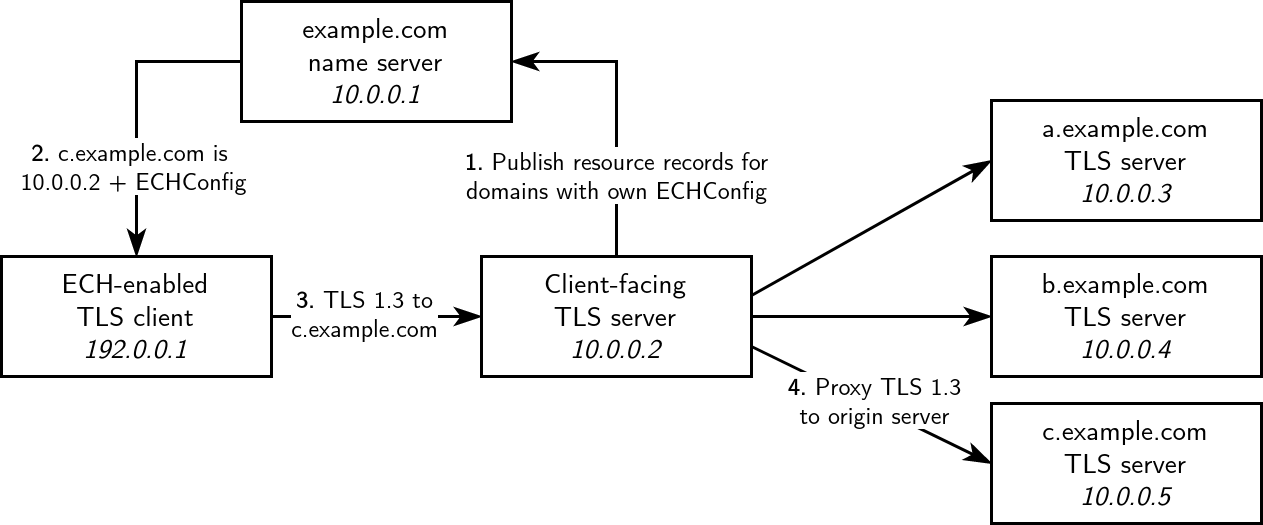
\includegraphics[width=160mm]{images/ech-split-mode.png}}
\caption[Example ECH Split Mode deployment]{<>}
\label{ech_split_mode_figure}
\end{figure}








\section{Traffic Analysis}

\blindtext

\subsection{Correlation Attacks}

\blindtext

\subsection{Traffic Padding}

\blindtext








\section{Summary}

\blindtext
